% Provenance (never printed): cycle 3 "La planete Terre" (the shaping of
% landscapes: erosion, transport and deposition by running water; rivers
% from source to mouth; floods); see sources/book1/PROVENANCE.md.
% Book 1, grade 5, chapter 1.
\chapter{L'eau façonne les paysages}\label{ch:g5:water-shapes-the-land}

Toute la nuit, l'orage a tambouriné sur le toit de l'école. Le matin, le
ciel s'éclaircit, et Lena et Tom courent jusqu'au petit ruisseau derrière
la cour. Hier, il était clair et tranquille~: on pouvait compter les \omterm{def:g3:stones-pebbles-sand:pebble}{galets}
de son lit. Aujourd'hui, il est large, rapide et brun, couleur de chocolat
au lait. Il charrie des brindilles, des feuilles, et quelque chose qu'ils
ne peuvent pas voir grain par grain~: de la \omterm{def:g3:stones-pebbles-sand:sand}{boue} et du \omterm{def:g3:stones-pebbles-sand:sand}{sable}, arrachés à
ses berges et aux champs situés en amont.

«~Où va toute cette \omterm{def:g3:stones-pebbles-sand:sand}{boue}~?~» demande Tom. Vers l'aval, un peu plus loin à
chaque minute. Le ruisseau emporte la terre, grain par grain. Dans ce
chapitre, nous suivons ces grains, depuis la \omterm{def:g3:stones-pebbles-sand:rock}{roche} d'où ils viennent
jusqu'à l'endroit où ils se déposent.

\begin{omfigure}
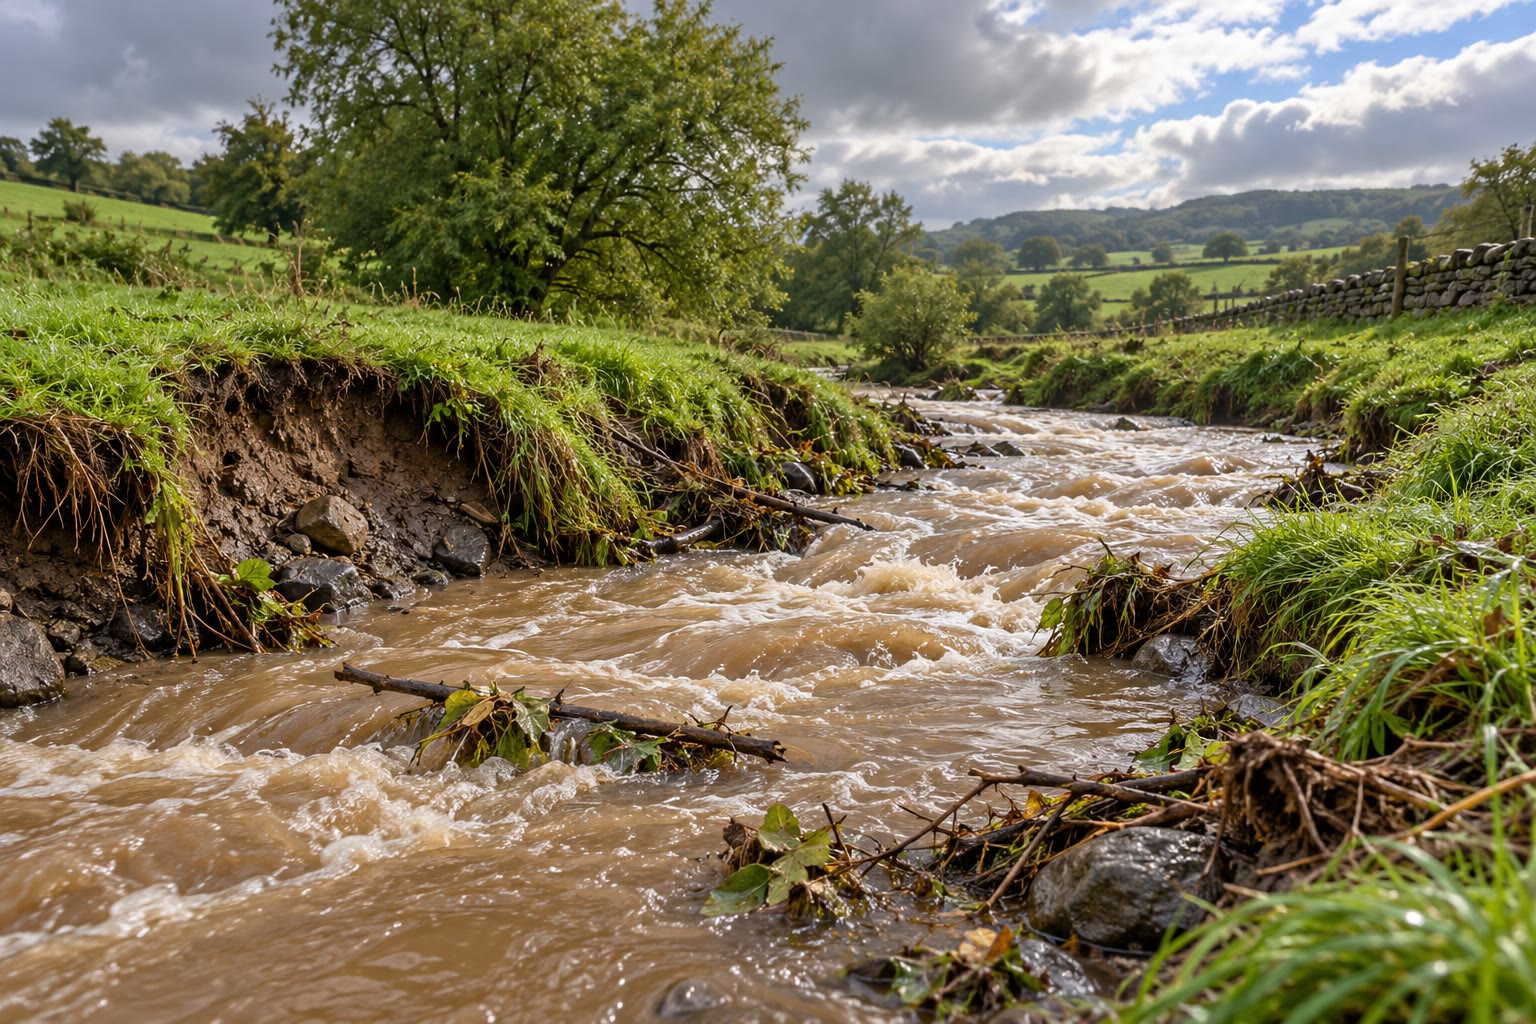
\includegraphics[width=0.5\linewidth]{images/book1/ai/g5-brown-stream.jpg}

{\small Un ruisseau au lendemain d'un orage~: l'eau est brune de la \omterm{def:g3:stones-pebbles-sand:sand}{boue} et
du \omterm{def:g3:stones-pebbles-sand:sand}{sable} qu'elle transporte.}
\end{omfigure}

\begin{recall}
La \omterm{def:g3:stones-pebbles-sand:rock}{roche} est le matériau dur de la Terre~; brisée en morceaux, elle donne
des cailloux, des \omterm{def:g3:stones-pebbles-sand:pebble}{galets} arrondis par l'eau, du \omterm{def:g3:stones-pebbles-sand:sand}{sable} dont nous voyons les
grains un par un, et de la \omterm{def:g3:stones-pebbles-sand:sand}{boue} dont les grains sont trop petits pour être
vus (\cref{ch:g3:stones-pebbles-sand}). Une \omterm{def:g1:landscapes-around-us:water}{rivière} coule tout le temps
dans un long chenal, des terres hautes jusqu'à un \omterm{def:g1:landscapes-around-us:water}{lac} ou jusqu'à la \omterm{def:g2:water-on-earth:ocean}{mer}
(\cref{ch:g1:landscapes-around-us}). La \omterm{def:g4:clouds-rain-snow:precipitation}{pluie} qui tombe sur les terres
ruisselle jusque dans les ruisseaux et les \omterm{def:g1:landscapes-around-us:water}{rivières}, qui ramènent l'eau à
la \omterm{def:g2:water-on-earth:ocean}{mer} (\cref{ch:g2:water-on-earth}).
\end{recall}

\section{La roche se brise sur place}

Même la \omterm{def:g3:stones-pebbles-sand:rock}{roche} la plus dure ne dure pas éternellement. Là où elle est à
l'air libre, sous le soleil, la \omterm{def:g4:clouds-rain-snow:precipitation}{pluie} et le gel, elle se fissure et
s'effrite lentement.

\begin{definition}[Altération]\label{def:g5:water-shapes-the-land:weathering}
L'\emph{altération}\index{alteration@altération} est la lente
désagrégation de la \omterm{def:g3:stones-pebbles-sand:rock}{roche} sur place, par le gel, par l'eau, par les racines
des plantes, et par la chaleur et le froid. La \omterm{def:g3:stones-pebbles-sand:rock}{roche} est brisée en
morceaux, mais les morceaux restent sur place.
\end{definition}

Le gel est l'un des outils les plus puissants de l'\omterm{def:g5:water-shapes-the-land:weathering}{altération}. L'eau de
\omterm{def:g4:clouds-rain-snow:precipitation}{pluie} s'infiltre dans une fine fissure de la \omterm{def:g3:stones-pebbles-sand:rock}{roche}. Par une nuit froide,
elle gèle, et l'eau qui gèle prend un peu plus de place~: la glace pousse
sur les bords de la fissure et l'élargit un tout petit peu. Le lendemain,
la glace fond, un peu plus d'eau s'infiltre, et la nuit suivante, elle
gèle de nouveau. Au bout de nombreux hivers, un morceau de \omterm{def:g3:stones-pebbles-sand:rock}{roche} se
détache.

\begin{omfigure}
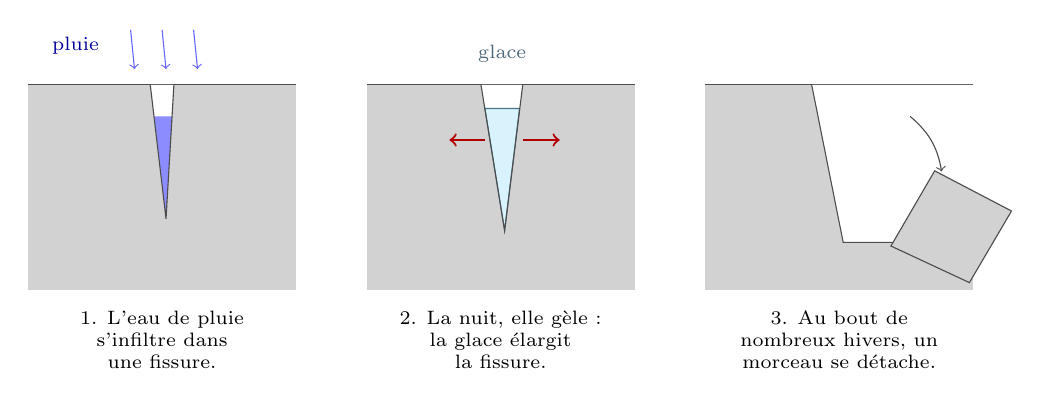
\begin{tikzpicture}[x=1cm, y=1cm, font=\scriptsize]
  \foreach \i/\t in {0/{1. L'eau de pluie\\s'infiltre dans\\une fissure.},
                     4.3/{2. La nuit, elle gèle~:\\la glace élargit\\la fissure.},
                     8.6/{3. Au bout de\\nombreux hivers, un\\morceau se détache.}} {
    \begin{scope}[xshift=\i cm]
      \fill[gray!35] (0,0) rectangle (3.4,2.6);
      \draw[gray!60!black] (0,2.6) -- (3.4,2.6);
      \node[align=center, anchor=north] at (1.7,-0.15) {\t};
    \end{scope}
  }
  % panel 1: thin crack with water
  \fill[white] (1.55,2.6) -- (1.75,0.9) -- (1.85,2.6) -- cycle;
  \fill[blue!45] (1.6,2.2) -- (1.75,0.9) -- (1.83,2.2) -- cycle;
  \draw[gray!60!black] (1.55,2.6) -- (1.75,0.9) -- (1.85,2.6);
  \foreach \x in {1.3,1.7,2.1} \draw[blue!60, ->] (\x,3.3) -- (\x+0.05,2.8);
  \node[blue!60!black] at (0.6,3.1) {pluie};
  % panel 2: wider crack with ice
  \begin{scope}[xshift=4.3cm]
    \fill[white] (1.45,2.6) -- (1.75,0.75) -- (1.98,2.6) -- cycle;
    \fill[cyan!15] (1.5,2.3) -- (1.75,0.75) -- (1.94,2.3) -- cycle;
    \draw[cyan!50!black] (1.5,2.3) -- (1.75,0.75) -- (1.94,2.3) -- cycle;
    \draw[gray!60!black] (1.45,2.6) -- (1.75,0.75) -- (1.98,2.6);
    \draw[red!70!black, thick, <-] (1.05,1.9) -- (1.5,1.9);
    \draw[red!70!black, thick, ->] (1.98,1.9) -- (2.45,1.9);
    \node[cyan!40!black] at (1.72,3.0) {glace};
  \end{scope}
  % panel 3: broken block
  \begin{scope}[xshift=8.6cm]
    \fill[white] (1.35,2.6) -- (1.75,0.6) -- (3.4,0.6) -- (3.4,2.6) -- cycle;
    \draw[gray!60!black] (1.35,2.6) -- (1.75,0.6) -- (3.4,0.6);
    \fill[gray!35, draw=gray!60!black, rotate around={-25:(2.9,0.3)}]
      (2.3,0.3) -- (2.4,1.4) -- (3.5,1.35) -- (3.4,0.3) -- cycle;
    \draw[gray!60!black, ->] (2.6,2.2) to[bend left=20] (3.0,1.5);
  \end{scope}
\end{tikzpicture}

{\small Le gel brise la \omterm{def:g3:stones-pebbles-sand:rock}{roche}. À chaque nuit de gel, la glace d'une fissure
pousse un peu~; au bout de nombreux hivers, la fissure est assez large pour
qu'un morceau se détache.}
\end{omfigure}

Au pied d'une paroi de \omterm{def:g3:stones-pebbles-sand:rock}{roche} nue, haut dans la \omterm{def:g1:landscapes-around-us:landform}{montagne}, les morceaux
détachés par le gel glissent, dégringolent et s'entassent en une pente de
cailloux pointus. Ils ne sont pas arrondis~: aucune eau ne les a encore
roulés.

\begin{omfigure}
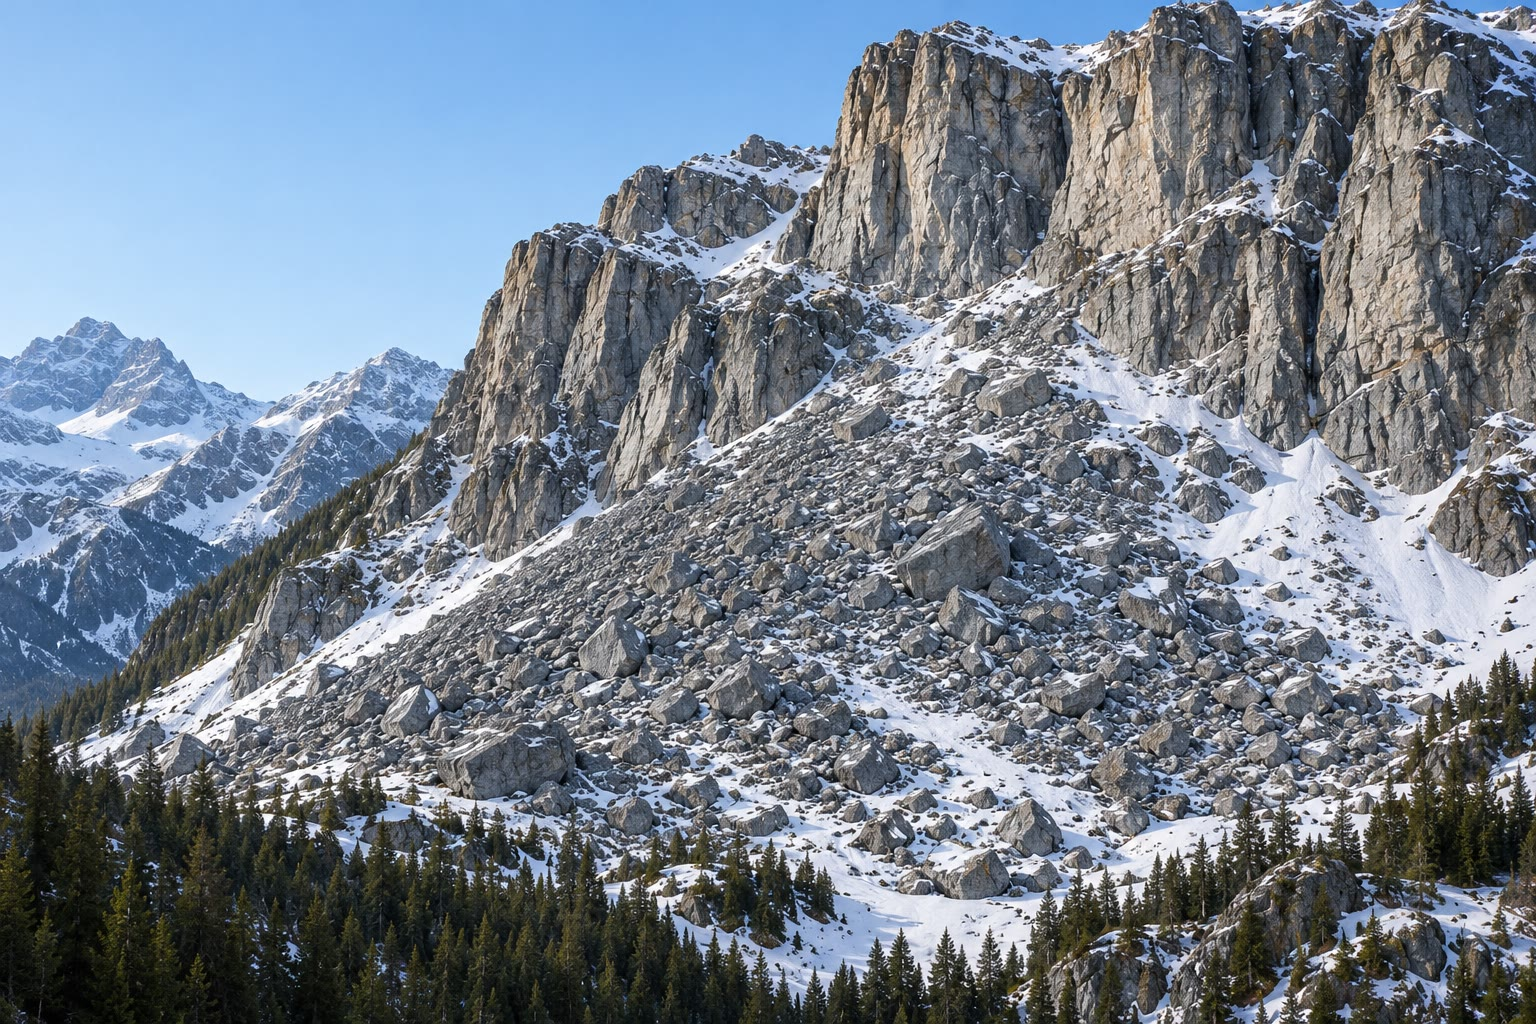
\includegraphics[width=0.5\linewidth]{images/book1/ai/g5-frost-scree.jpg}

{\small Au pied d'une paroi de \omterm{def:g1:landscapes-around-us:landform}{montagne}, une pente de cailloux aux arêtes
vives détachés par le gel, vue de l'autre côté de la \omterm{def:g1:landscapes-around-us:landform}{vallée}.}
\end{omfigure}

Les plantes aident aussi. Une racine d'arbre se glisse dans une fissure et,
en grossissant année après année, elle fend la \omterm{def:g3:stones-pebbles-sand:rock}{roche} comme un coin qui
avance lentement. L'eau de \omterm{def:g4:clouds-rain-snow:precipitation}{pluie} elle-même ramollit lentement certaines
\omterm{def:g3:stones-pebbles-sand:rock}{roches} et les transforme en argile et en \omterm{def:g3:stones-pebbles-sand:sand}{sable}~: c'est ainsi que le sol
reçoit ses grains minéraux.

\section{L'eau emporte les morceaux}

Une fois la \omterm{def:g3:stones-pebbles-sand:rock}{roche} brisée, les morceaux peuvent bouger. Encore faut-il que quelque chose les transporte.

\begin{definition}[Érosion]\label{def:g5:water-shapes-the-land:erosion}
L'\emph{érosion}\index{erosion@érosion} est l'usure des terres et
l'enlèvement des morceaux de \omterm{def:g3:stones-pebbles-sand:rock}{roche}, surtout par l'eau qui ruisselle, mais
aussi par le vent, par la glace et par les vagues de la \omterm{def:g2:water-on-earth:ocean}{mer}.
\end{definition}

L'eau courante fait l'essentiel du travail. La \omterm{def:g4:clouds-rain-snow:precipitation}{pluie} entraîne la terre et
les grains le long des pentes jusque dans les ruisseaux~; les ruisseaux en
arrachent davantage à leurs propres berges, comme le ruisseau de Tom et
Lena après l'orage. Plus l'eau coule vite, plus elle peut transporter, et
plus les morceaux qu'elle déplace sont gros~: un ruisseau calme ne
transporte que de la \omterm{def:g3:stones-pebbles-sand:sand}{boue} fine~; un ruisseau en \omterm{def:g5:water-shapes-the-land:flood}{crue} roule des \omterm{def:g3:stones-pebbles-sand:pebble}{galets} et
même des blocs sur son lit.

En chemin, les cailloux se cognent les uns contre les autres et contre le
lit. Leurs angles se cassent, et ils deviennent des \omterm{def:g3:stones-pebbles-sand:pebble}{galets} arrondis, puis
des grains de plus en plus petits~: du \omterm{def:g3:stones-pebbles-sand:sand}{sable} et de la \omterm{def:g3:stones-pebbles-sand:sand}{boue}.

Le vent fait le même travail dans les endroits secs, où rien ne retient le
\omterm{def:g3:stones-pebbles-sand:sand}{sable}~: il l'accumule en dunes. La glace, en \omterm{def:g1:landscapes-around-us:landform}{montagne} et près des \omterm{def:g3:continents-and-oceans:poles}{pôles},
entraîne des cailloux sous son énorme poids. Sur la \omterm{def:g1:landscapes-around-us:water}{côte}, les vagues
frappent les falaises et font rouler en va-et-vient les \omterm{def:g3:stones-pebbles-sand:pebble}{galets} de la plage.

\begin{remark}[Combien~?]\label{rem:g5:water-shapes-the-land:how-much}
Ensemble, tous les fleuves du monde apportent à la \omterm{def:g2:water-on-earth:ocean}{mer} plus de
12 milliards de tonnes de \omterm{def:g3:stones-pebbles-sand:sand}{boue} et de \omterm{def:g3:stones-pebbles-sand:sand}{sable} chaque année. Cela fait environ
un milliard de tonnes chaque mois.
% ledger: syvitski:modern-flux
\end{remark}

\section{L'eau dépose les morceaux}

Une \omterm{def:g1:landscapes-around-us:water}{rivière} ne peut pas transporter sa charge indéfiniment. Là où elle
ralentit, elle n'a plus la force de déplacer ses plus gros grains, et ils
se déposent sur le lit.

\begin{definition}[Dépôt]\label{def:g5:water-shapes-the-land:deposition}
Le \emph{dépôt}\index{depot@dépôt} est la mise en place, là où ils
ralentissent et s'arrêtent, des morceaux de \omterm{def:g3:stones-pebbles-sand:rock}{roche} transportés par l'eau,
le vent ou la glace.
\end{definition}

Les morceaux les plus lourds se déposent en premier~: les \omterm{def:g3:stones-pebbles-sand:pebble}{galets} tombent là
où le courant faiblit un peu, le \omterm{def:g3:stones-pebbles-sand:sand}{sable} là où il ralentit davantage, et la
\omterm{def:g3:stones-pebbles-sand:sand}{boue} fine seulement là où l'eau est presque immobile, dans un \omterm{def:g1:landscapes-around-us:water}{lac} ou dans
la \omterm{def:g2:water-on-earth:ocean}{mer}. C'est pourquoi le lit d'une \omterm{def:g1:landscapes-around-us:water}{rivière} est couvert de \omterm{def:g3:stones-pebbles-sand:pebble}{galets} en
\omterm{def:g1:landscapes-around-us:landform}{montagne}, et de \omterm{def:g3:stones-pebbles-sand:sand}{sable} ou de \omterm{def:g3:stones-pebbles-sand:sand}{boue} près de la \omterm{def:g2:water-on-earth:ocean}{mer}.

L'\omterm{def:g5:water-shapes-the-land:weathering}{altération}, l'\omterm{def:g5:water-shapes-the-land:erosion}{érosion} et le \omterm{def:g5:water-shapes-the-land:deposition}{dépôt} sont trois étapes d'un même long
voyage~: la \omterm{def:g3:stones-pebbles-sand:rock}{roche} est brisée sur place, ses morceaux sont emportés, et ils
sont déposés ailleurs. Lentement, l'eau déplace les \omterm{def:g1:landscapes-around-us:landform}{montagnes}, grain par
grain, jusqu'aux \omterm{def:g1:landscapes-around-us:landform}{plaines} et jusqu'à la \omterm{def:g2:water-on-earth:ocean}{mer}.

\begin{method}[Nommer ce que fait l'eau]\label{met:g5:water-shapes-the-land:naming}
Pour nommer ce qui arrive à la \omterm{def:g3:stones-pebbles-sand:rock}{roche} sur une image ou dans un récit,
pose-toi trois questions~:
\begin{enumerate}
  \item La \omterm{def:g3:stones-pebbles-sand:rock}{roche} est-elle brisée, mais les morceaux restent-ils où ils
        sont~? C'est l'\emph{\omterm{def:g5:water-shapes-the-land:weathering}{altération}}.
  \item Les morceaux sont-ils usés et emportés~? C'est
        l'\emph{\omterm{def:g5:water-shapes-the-land:erosion}{érosion}}.
  \item Les morceaux se posent-ils et s'entassent-ils~? C'est le
        \emph{\omterm{def:g5:water-shapes-the-land:deposition}{dépôt}}.
\end{enumerate}
\end{method}

\begin{example}[Le ruisseau après l'orage]\label{ex:g5:water-shapes-the-land:stream}
L'eau brune du ruisseau de Tom et Lena transporte de la \omterm{def:g3:stones-pebbles-sand:sand}{boue} arrachée à ses
berges~: c'est l'\omterm{def:g5:water-shapes-the-land:erosion}{érosion}. Une semaine plus tard, le ruisseau est de nouveau
clair, et une fine couche de \omterm{def:g3:stones-pebbles-sand:sand}{boue} couvre le fond de la mare tranquille au
bout de la cour~: c'est le \omterm{def:g5:water-shapes-the-land:deposition}{dépôt}.
\end{example}

\section{Une rivière de sa source à son embouchure}

Toute \omterm{def:g1:landscapes-around-us:water}{rivière} a un commencement et une fin.

\begin{definition}[Source, embouchure et affluent]\label{def:g5:water-shapes-the-land:source-mouth}
La \emph{source}\index{source (d'un cours d'eau)} d'une \omterm{def:g1:landscapes-around-us:water}{rivière} est
l'endroit où elle commence~: une source d'eau qui jaillit du sol, un
glacier qui fond, ou une terre haute et humide où naissent de nombreux
petits ruisseaux. Son \emph{embouchure}\index{embouchure} est l'endroit où
elle se termine, en se jetant dans la \omterm{def:g2:water-on-earth:ocean}{mer}, dans un \omterm{def:g1:landscapes-around-us:water}{lac} ou dans une \omterm{def:g1:landscapes-around-us:water}{rivière}
plus grande. Un \emph{affluent}\index{affluent} est une \omterm{def:g1:landscapes-around-us:water}{rivière} plus
petite qui se jette dans une plus grande.
\end{definition}

Tout au long de son chemin, une \omterm{def:g1:landscapes-around-us:water}{rivière} change. Nous partageons sa
longueur en trois parties~: son cours supérieur, son cours moyen et son
cours inférieur.

\begin{omfigure}
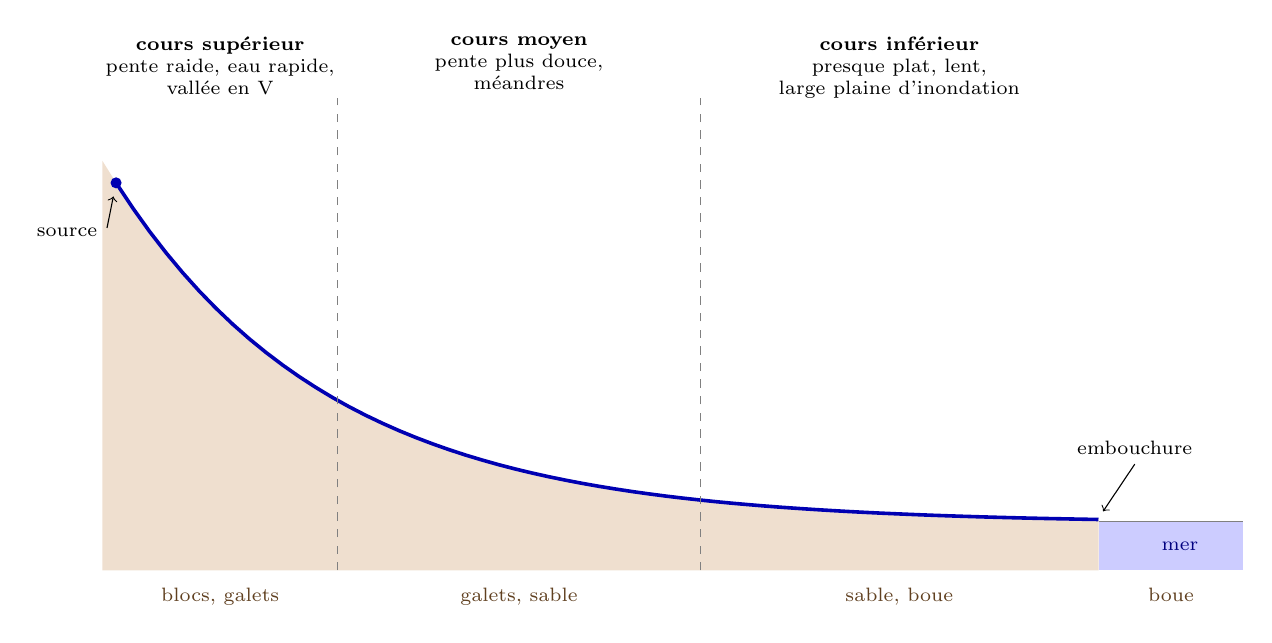
\begin{tikzpicture}[x=1.15cm, y=1cm, font=\scriptsize]
  % ground
  \fill[brown!25] (0,-0.6) -- plot[domain=0:11, samples=60]
    (\x,{4.6*exp(-\x/2.4)}) -- (11,-0.6) -- cycle;
  % sea
  \fill[blue!20] (11,-0.6) rectangle (12.6,0.02);
  \draw[blue!70!black, line width=1.3pt] plot[domain=0.15:11, samples=60]
    (\x,{4.6*exp(-\x/2.4)});
  \draw[gray] (11,0.02) -- (12.6,0.02);
  \node[blue!50!black] at (11.9,-0.3) {mer};
  % course limits
  \foreach \x in {2.6,6.6} \draw[gray, dashed] (\x,-0.6) -- (\x,5.4);
  \node[align=center, anchor=north] at (1.3,6.3) {\textbf{cours supérieur}\\pente raide, eau rapide,\\vallée en V};
  \node[align=center, anchor=north] at (4.6,6.3) {\textbf{cours moyen}\\pente plus douce,\\méandres};
  \node[align=center, anchor=north] at (8.8,6.3) {\textbf{cours inférieur}\\presque plat, lent,\\large plaine d'inondation};
  % source and mouth
  \fill[blue!70!black] (0.15,{4.6*exp(-0.15/2.4)}) circle (2pt);
  \node[anchor=east] at (0.05,3.7) {source};
  \draw[->] (0.05,3.75) -- (0.12,4.15);
  \node[anchor=south] at (11.4,0.75) {embouchure};
  \draw[->] (11.4,0.75) -- (11.05,0.15);
  % grain sizes
  \node[anchor=north, align=center, text=brown!50!black] at (1.3,-0.7) {blocs, galets};
  \node[anchor=north, align=center, text=brown!50!black] at (4.6,-0.7) {galets, sable};
  \node[anchor=north, align=center, text=brown!50!black] at (8.8,-0.7) {sable, boue};
  \node[anchor=north, align=center, text=brown!50!black] at (11.8,-0.7) {boue};
\end{tikzpicture}

{\small Le profil en long d'une \omterm{def:g1:landscapes-around-us:water}{rivière}, de sa \omterm{def:g5:water-shapes-the-land:source-mouth}{source} à son \omterm{def:g5:water-shapes-the-land:source-mouth}{embouchure} (les
hauteurs sont très exagérées). En dessous~: ce qui couvre son lit.}
\end{omfigure}

Dans son \emph{cours supérieur}, en \omterm{def:g1:landscapes-around-us:landform}{montagne}, la \omterm{def:g1:landscapes-around-us:water}{rivière} est jeune et
pentue. Son eau dévale, roule des blocs sur son lit et creuse la \omterm{def:g3:stones-pebbles-sand:rock}{roche} vers
le bas. Elle creuse une \omterm{def:g1:landscapes-around-us:landform}{vallée} étroite aux versants raides, en forme de
lettre V.

Dans son \emph{cours moyen}, la pente est plus douce. La \omterm{def:g1:landscapes-around-us:water}{rivière} oscille
d'un côté à l'autre en grandes boucles.

\begin{definition}[Méandre]\label{def:g5:water-shapes-the-land:meander}
Un \emph{méandre}\index{meandre@méandre} est une boucle d'une \omterm{def:g1:landscapes-around-us:water}{rivière} qui
serpente sur un fond de \omterm{def:g1:landscapes-around-us:landform}{vallée} plat.
\end{definition}

Un \omterm{def:g5:water-shapes-the-land:meander}{méandre} ne reste pas immobile~: il se déplace. À l'extérieur de chaque
courbe, l'eau coule vite et profond~: elle ronge la berge, qui devient une
petite falaise. À l'intérieur de la courbe, l'eau coule lentement~: elle
dépose du \omterm{def:g3:stones-pebbles-sand:sand}{sable} et des \omterm{def:g3:stones-pebbles-sand:pebble}{graviers}, qui forment une plage en pente douce.
Année après année, la berge extérieure recule, la plage intérieure grandit,
et la boucle s'élargit de plus en plus.

\begin{omfigure}
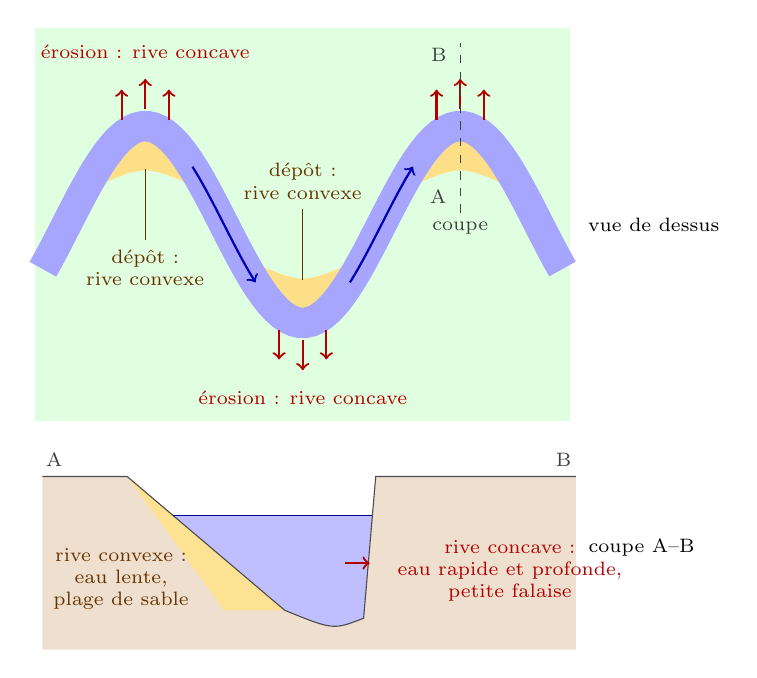
\begin{tikzpicture}[x=1cm, y=1cm, font=\scriptsize]
  % ---- map view ----
  \fill[green!12] (-0.4,-2.5) rectangle (6.4,2.5);
  % sand on the inner banks (drawn first, the river covers its edge)
  \foreach \c/\s in {1/1, 3/-1, 5/1}
    \fill[yellow!50!orange!45] (\c-0.6,\s*0.5) .. controls (\c,\s*1.5) ..
      (\c+0.6,\s*0.5) .. controls (\c,\s*0.75) .. cycle;
  % the river
  \draw[blue!35, line width=11pt] plot[domain=-0.3:6.3, samples=90]
    (\x,{1.25*sin(\x*90)});
  \draw[blue!70!black, ->, thick] plot[domain=1.6:2.4, samples=10]
    (\x,{1.25*sin(\x*90)});
  \draw[blue!70!black, ->, thick] plot[domain=3.6:4.4, samples=10]
    (\x,{1.25*sin(\x*90)});
  % erosion on the outer banks
  \foreach \c/\s in {1/1, 3/-1, 5/1}
    \foreach \d in {-0.3,0,0.3}
      \draw[red!70!black, thick, ->] (\c+\d,{\s*(1.25*cos(\d*90)+0.22)})
        -- (\c+\d,{\s*(1.25*cos(\d*90)+0.6)});
  \node[red!70!black] at (1,2.2) {érosion~: rive concave};
  \node[red!70!black] at (3,-2.2) {érosion~: rive concave};
  \node[orange!40!black, align=center] (d1) at (1,-0.55) {dépôt~:\\rive convexe};
  \node[orange!40!black, align=center] (d2) at (3,0.55) {dépôt~:\\rive convexe};
  \draw[orange!40!black] (d1.north) -- (1,0.7);
  \draw[orange!40!black] (d2.south) -- (3,-0.7);
  \draw[gray!50!black, dashed] (5,0.15) -- (5,2.3);
  \node[gray!50!black, anchor=north] at (5,0.15) {coupe};
  \node[gray!50!black, anchor=east] at (4.95,0.35) {A};
  \node[gray!50!black, anchor=east] at (4.95,2.15) {B};
  \node[anchor=west] at (6.5,0) {vue de dessus};
  % ---- cut ----
  \begin{scope}[yshift=-4.1cm, xscale=0.77]
    \fill[brown!25] (-0.4,-1.3) -- (-0.4,0.9) -- (1,0.9) -- (3.6,-0.8)
      .. controls (4.4,-1.05) .. (4.9,-0.9) -- (5.1,0.9) -- (8.4,0.9)
      -- (8.4,-1.3) -- cycle;
    \fill[blue!25] (1.75,0.4) -- (3.6,-0.8) .. controls (4.4,-1.05) .. (4.9,-0.9)
      -- (5.04,0.4) -- cycle;
    \fill[yellow!50!orange!40] (1,0.9) -- (3.6,-0.8) -- (2.6,-0.8) -- cycle;
    \draw[gray!60!black] (-0.4,0.9) -- (1,0.9) -- (3.6,-0.8)
      .. controls (4.4,-1.05) .. (4.9,-0.9) -- (5.1,0.9) -- (8.4,0.9);
    \draw[blue!60!black] (1.75,0.4) -- (5.04,0.4);
    \node[orange!40!black, align=center] at (0.9,-0.4) {rive convexe~:\\eau lente,\\plage de sable};
    \node[red!70!black, align=center, anchor=west] at (5.3,-0.3) {rive concave~:\\eau rapide et profonde,\\petite falaise};
    \draw[red!70!black, thick, ->] (4.6,-0.2) -- (5.0,-0.2);
    \node[gray!50!black, anchor=south] at (-0.2,0.9) {A};
    \node[gray!50!black, anchor=south] at (8.2,0.9) {B};
    \node[anchor=west] at (8.45,0) {coupe A--B};
  \end{scope}
\end{tikzpicture}

{\small Un \omterm{def:g5:water-shapes-the-land:meander}{méandre} vu de dessus, et en coupe le long de la ligne en tirets
A--B. L'eau use la rive extérieure (concave) de chaque courbe et dépose du
\omterm{def:g3:stones-pebbles-sand:sand}{sable} sur la rive intérieure (convexe)~: la boucle se déplace lentement.}
\end{omfigure}

Parfois, deux boucles se rapprochent tellement que, pendant une \omterm{def:g5:water-shapes-the-land:flood}{crue}, la
\omterm{def:g1:landscapes-around-us:water}{rivière} perce l'étroit pédoncule de terre qui les sépare et prend le
raccourci. L'ancienne boucle reste en arrière sous la forme d'un \omterm{def:g1:landscapes-around-us:water}{lac} en
croissant.

\begin{omfigure}
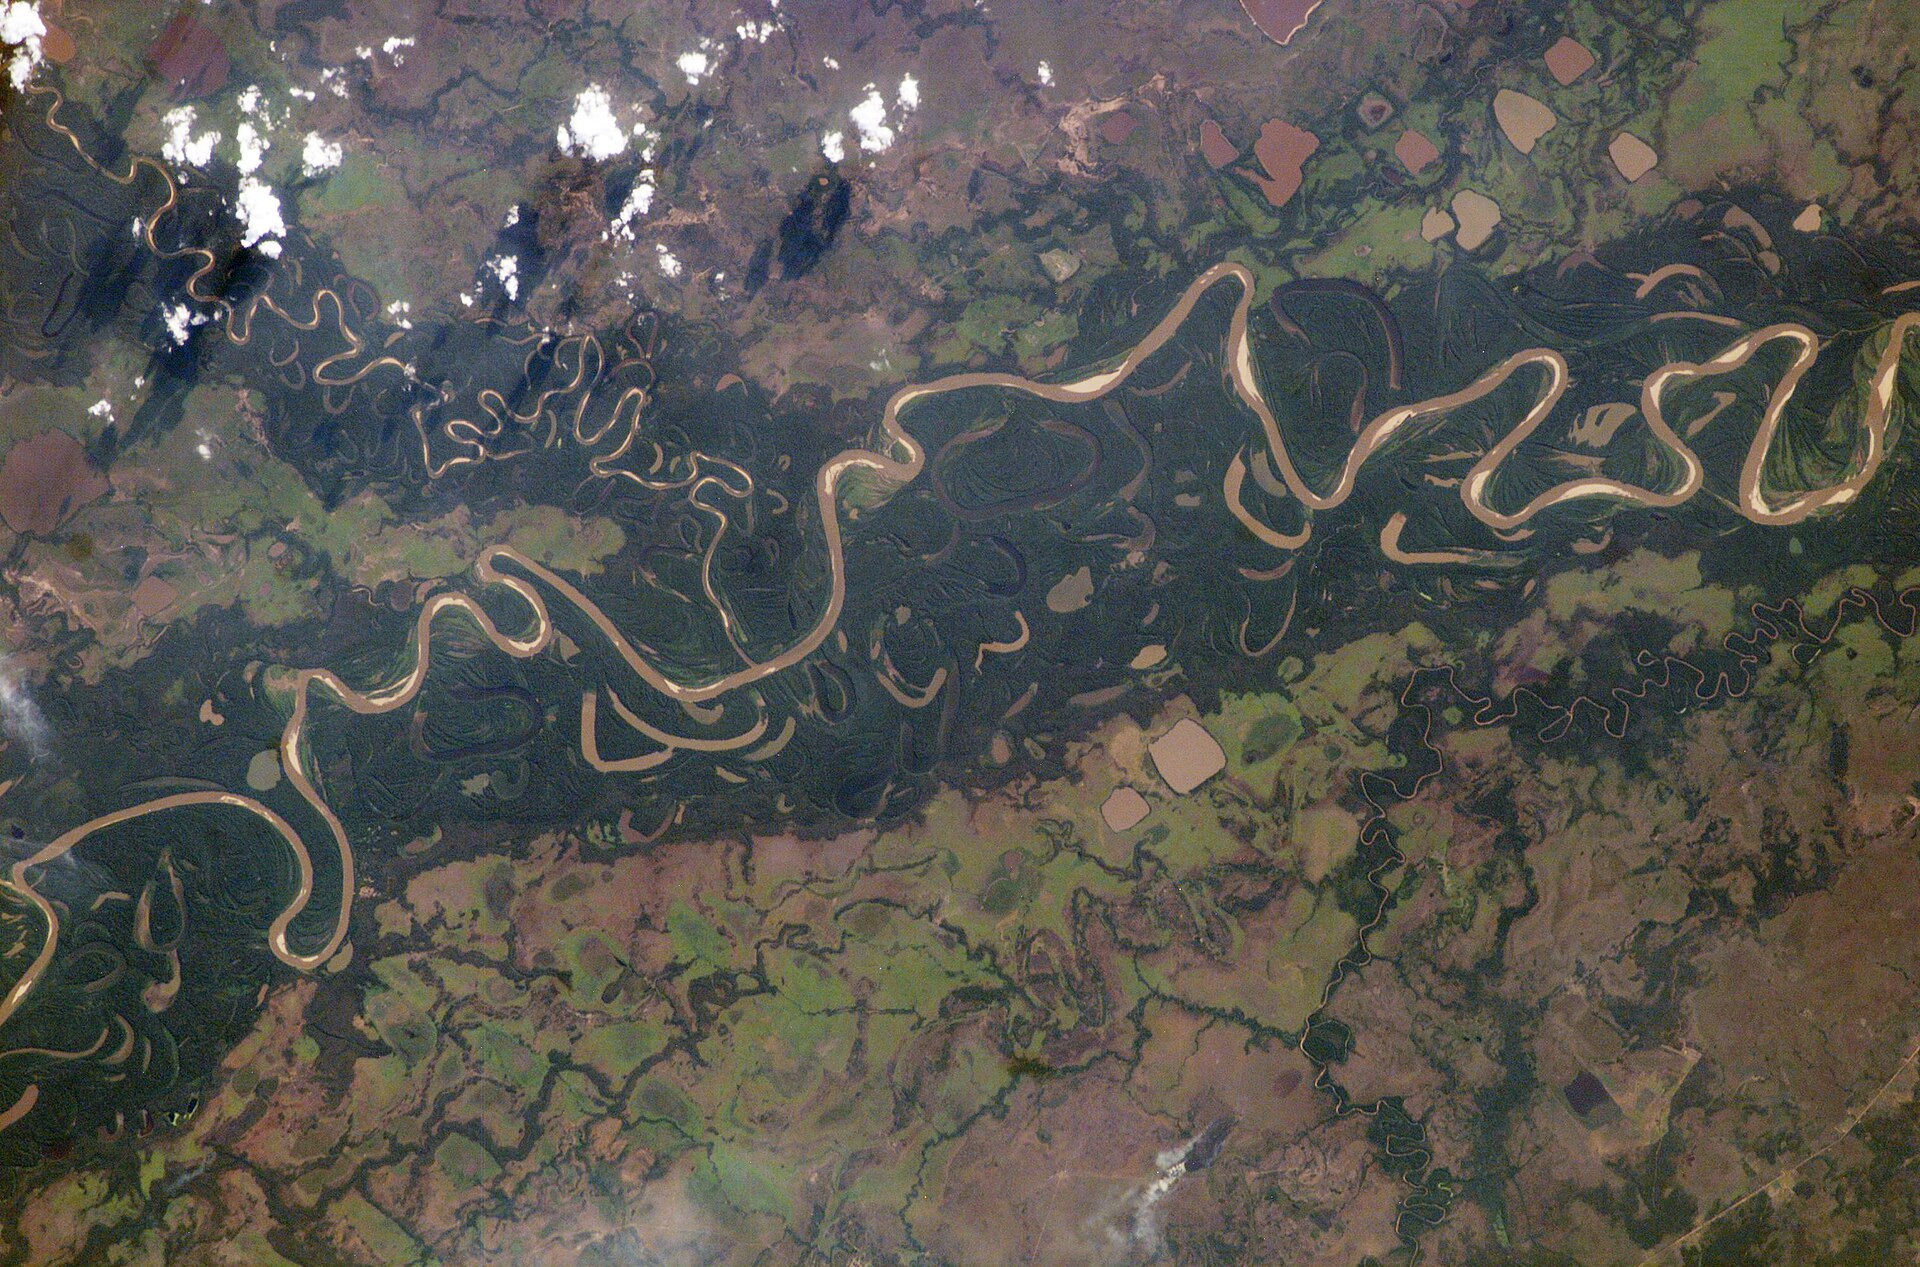
\includegraphics[width=0.52\linewidth]{images/book1/g5-mamore-meanders.jpg}

{\small Le Mamoré, dans les \omterm{def:g1:landscapes-around-us:landform}{plaines} basses de la Bolivie en Amérique du Sud,
vu depuis la Station spatiale internationale. La \omterm{def:g1:landscapes-around-us:water}{rivière} brune serpente en
\omterm{def:g5:water-shapes-the-land:meander}{méandres} à travers la forêt. Photographie~: NASA (domaine public).}\label{fig:g5:water-shapes-the-land:mamore}
% ledger: nasa:mamore-meanders
\end{omfigure}

Dans son \emph{cours inférieur}, le terrain est presque plat. La \omterm{def:g1:landscapes-around-us:water}{rivière}
coule lentement sur un fond de \omterm{def:g1:landscapes-around-us:landform}{vallée} large et plat, fait de la \omterm{def:g3:stones-pebbles-sand:sand}{boue} et du
\omterm{def:g3:stones-pebbles-sand:sand}{sable} qu'elle a elle-même déposés pendant très longtemps.

\begin{omfigure}
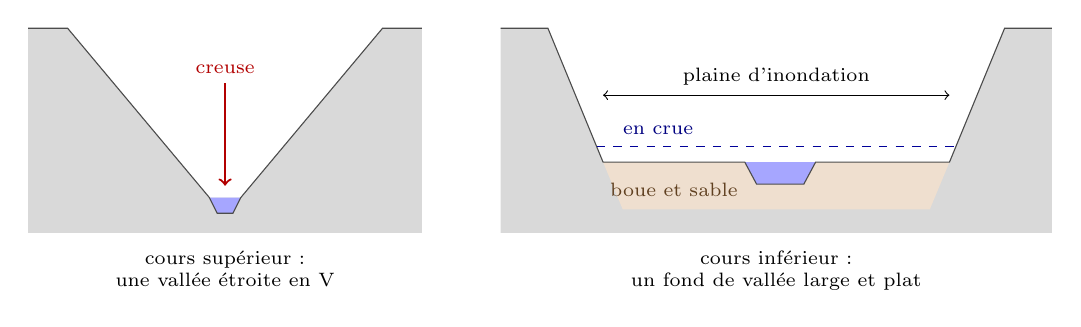
\begin{tikzpicture}[x=1cm, y=1cm, font=\scriptsize]
  % V-shaped valley
  \fill[gray!30] (0,0) -- (0,2.6) -- (0.5,2.6) -- (2.3,0.45) -- (2.7,0.45)
    -- (4.5,2.6) -- (5,2.6) -- (5,0) -- cycle;
  \fill[blue!35] (2.3,0.45) -- (2.4,0.25) -- (2.6,0.25) -- (2.7,0.45) -- cycle;
  \draw[gray!60!black] (0,2.6) -- (0.5,2.6) -- (2.3,0.45) -- (2.4,0.25)
    -- (2.6,0.25) -- (2.7,0.45) -- (4.5,2.6) -- (5,2.6);
  \draw[red!70!black, thick, ->] (2.5,1.9) -- (2.5,0.6);
  \node[red!70!black, anchor=south] at (2.5,1.9) {creuse};
  \node[align=center, anchor=north] at (2.5,-0.1) {cours supérieur~:\\une vallée étroite en V};
  % floodplain
  \begin{scope}[xshift=6cm]
    \fill[gray!30] (0,0) -- (0,2.6) -- (0.6,2.6) -- (1.3,0.9) -- (5.7,0.9)
      -- (6.4,2.6) -- (7,2.6) -- (7,0) -- cycle;
    \fill[brown!25] (1.3,0.9) -- (1.55,0.3) -- (5.45,0.3) -- (5.7,0.9) -- cycle;
    \fill[blue!35] (3.1,0.9) -- (3.25,0.62) -- (3.85,0.62) -- (4,0.9) -- cycle;
    \draw[gray!60!black] (0,2.6) -- (0.6,2.6) -- (1.3,0.9) -- (3.1,0.9)
      -- (3.25,0.62) -- (3.85,0.62) -- (4,0.9) -- (5.7,0.9) -- (6.4,2.6) -- (7,2.6);
    \draw[blue!60!black, dashed] (1.22,1.1) -- (5.78,1.1);
    \node[blue!50!black, anchor=south] at (2.0,1.12) {en crue};
    \node[brown!50!black] at (2.2,0.55) {boue et sable};
    \draw[<->] (1.3,1.75) -- (5.7,1.75);
    \node[anchor=south] at (3.5,1.75) {plaine d'inondation};
    \node[align=center, anchor=north] at (3.5,-0.1) {cours inférieur~:\\un fond de vallée large et plat};
  \end{scope}
\end{tikzpicture}

{\small La \omterm{def:g1:landscapes-around-us:landform}{vallée} en coupe, en \omterm{def:g1:landscapes-around-us:landform}{montagne} et près de la \omterm{def:g2:water-on-earth:ocean}{mer} (pas à la même
échelle). En \omterm{def:g5:water-shapes-the-land:flood}{crue}, la \omterm{def:g1:landscapes-around-us:water}{rivière} s'étale sur toute sa \omterm{def:g5:water-shapes-the-land:flood}{plaine d'inondation}.}
\end{omfigure}

Enfin, la \omterm{def:g1:landscapes-around-us:water}{rivière} atteint son \omterm{def:g5:water-shapes-the-land:source-mouth}{embouchure}. Là, l'eau ralentit presque
complètement, et la \omterm{def:g1:landscapes-around-us:water}{rivière} dépose le reste de sa charge. Là où les vagues
et les marées de la \omterm{def:g2:water-on-earth:ocean}{mer} sont trop faibles pour tout emporter, la \omterm{def:g3:stones-pebbles-sand:sand}{boue} et
le \omterm{def:g3:stones-pebbles-sand:sand}{sable} s'accumulent, et une terre nouvelle avance dans la \omterm{def:g2:water-on-earth:ocean}{mer}.

\begin{definition}[Delta]\label{def:g5:water-shapes-the-land:delta}
Un \emph{delta}\index{delta} est une terre nouvelle et plate, construite par
une \omterm{def:g1:landscapes-around-us:water}{rivière} à son \omterm{def:g5:water-shapes-the-land:source-mouth}{embouchure} avec la \omterm{def:g3:stones-pebbles-sand:sand}{boue} et le \omterm{def:g3:stones-pebbles-sand:sand}{sable} qu'elle dépose. La
\omterm{def:g1:landscapes-around-us:water}{rivière} s'y divise en plusieurs bras qui s'étalent, souvent en forme
d'éventail.
\end{definition}

Le nom vient de la lettre grecque $\Delta$ (\omterm{def:g5:water-shapes-the-land:delta}{delta}), un triangle, parce que
le \omterm{def:g5:water-shapes-the-land:delta}{delta} du Nil, en Égypte, a cette forme.

Certaines \omterm{def:g1:landscapes-around-us:water}{rivières} se terminent sans \omterm{def:g5:water-shapes-the-land:delta}{delta}. Là où de fortes vagues et de
fortes marées balaient la \omterm{def:g3:stones-pebbles-sand:sand}{boue}, la \omterm{def:g1:landscapes-around-us:water}{rivière} se termine par une \omterm{def:g5:water-shapes-the-land:source-mouth}{embouchure}
large, en forme d'entonnoir, où la \omterm{def:g2:water-on-earth:ocean}{mer} entre et sort au rythme des
marées~: un \emph{estuaire}.

\begin{omfigure}
\begin{minipage}[b]{0.55\linewidth}\centering
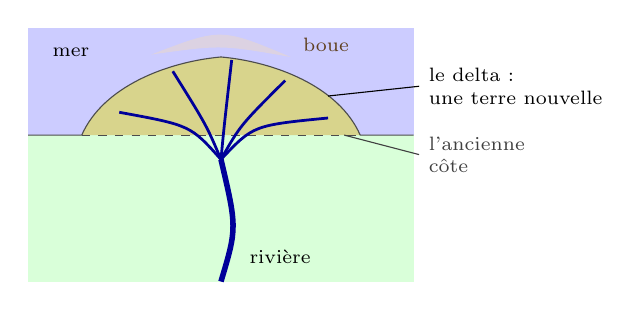
\begin{tikzpicture}[x=0.68cm, y=0.62cm, font=\scriptsize]
  \fill[blue!20] (-3.6,1.4) rectangle (3.6,3.6);
  \fill[green!15] (-3.6,-1.6) rectangle (3.6,1.4);
  % delta
  \fill[olive!35] (-2.6,1.4) .. controls (-2.2,2.4) and (-1,2.9)
    .. (0,3.0) .. controls (1,2.9) and (2.2,2.4) .. (2.6,1.4) -- cycle;
  \draw[gray!60!black] (-3.6,1.4) -- (-2.6,1.4) .. controls (-2.2,2.4) and
    (-1,2.9) .. (0,3.0) .. controls (1,2.9) and (2.2,2.4) .. (2.6,1.4) -- (3.6,1.4);
  \draw[gray!60!black, dashed] (-2.6,1.4) -- (2.6,1.4);
  % river and branches
  \draw[blue!60!black, line width=2pt] (0,-1.6) .. controls (0.3,-0.5) .. (0,0.9);
  \foreach \e in {-1.9,-0.9,0.2,1.2,2.0}
    \draw[blue!60!black, line width=1pt] (0,0.9) .. controls (\e*0.3,1.6) ..
      (\e,{2.95-0.3*\e*\e});
  % mud plume
  \fill[brown!30, opacity=0.5] (-1.3,3.05) .. controls (0,3.6) .. (1.3,3.0)
    .. controls (0,3.25) .. cycle;
  \node[align=center] at (-2.8,3.1) {mer};
  \node[anchor=west, brown!50!black] at (1.35,3.25) {boue};
  \node[anchor=west, align=left] at (3.7,2.4) {le delta~:\\une terre nouvelle};
  \draw (3.7,2.4) -- (2.0,2.2);
  \node[anchor=west, align=left, gray!50!black] at (3.7,1.0) {l'ancienne\\côte};
  \draw[gray!50!black] (3.7,1.0) -- (2.3,1.4);
  \node[anchor=west] at (0.35,-1.1) {rivière};
\end{tikzpicture}
\end{minipage}\hfill
\begin{minipage}[b]{0.3\linewidth}\centering
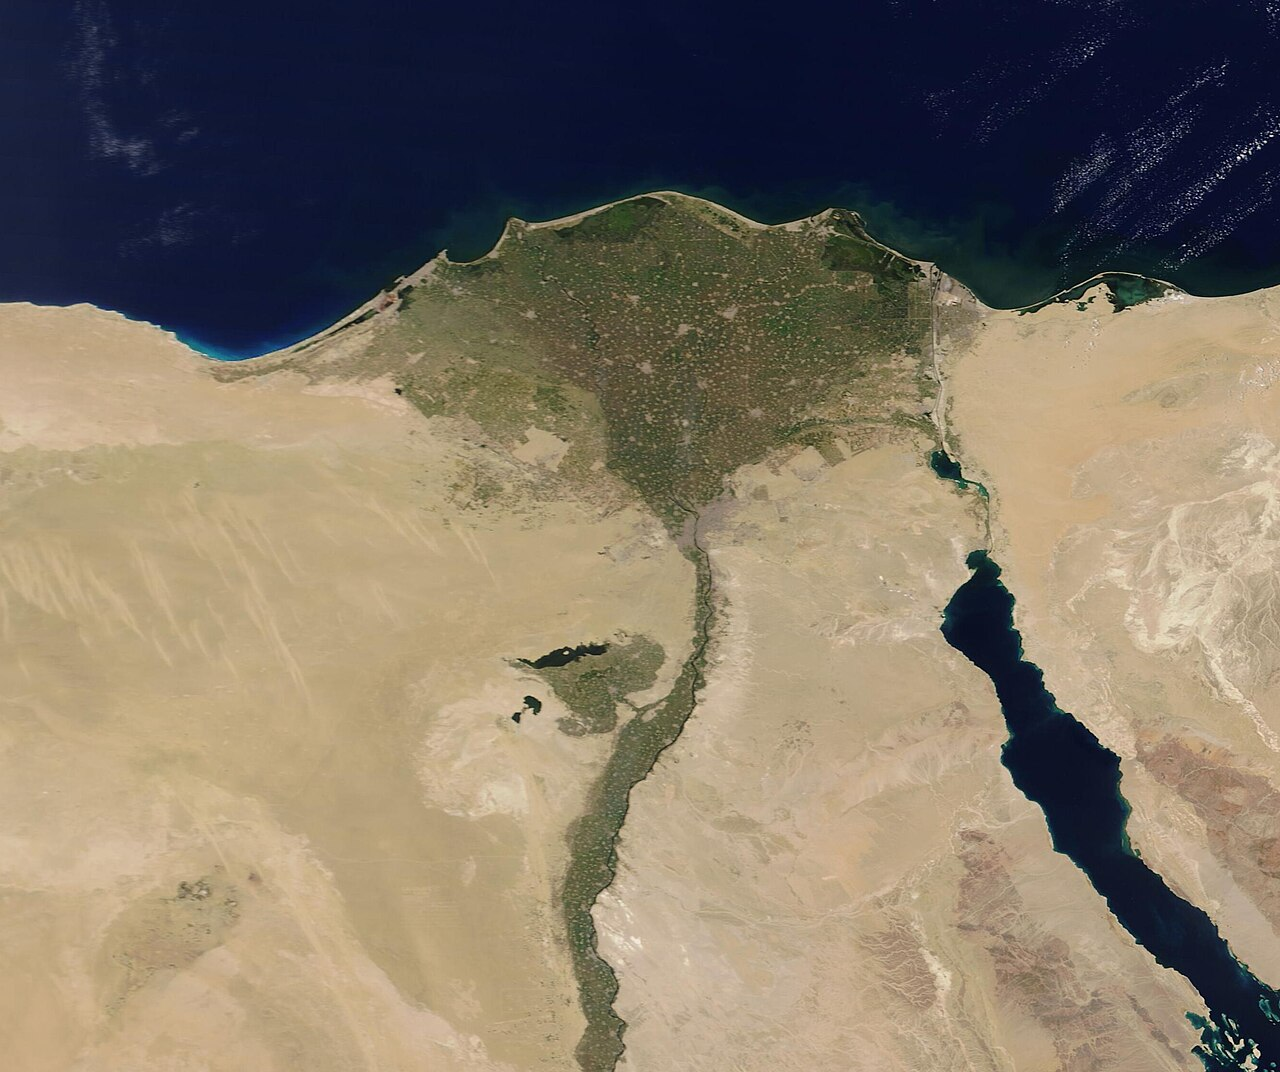
\includegraphics[width=\linewidth]{images/book1/g5-nile-delta-modis.jpg}
\end{minipage}

{\small À gauche~: un \omterm{def:g5:water-shapes-the-land:delta}{delta} vu de dessus~; la \omterm{def:g3:stones-pebbles-sand:sand}{boue} et le \omterm{def:g3:stones-pebbles-sand:sand}{sable} déposés par
les bras construisent une terre nouvelle au-delà de l'ancienne \omterm{def:g1:landscapes-around-us:water}{côte}. À
droite~: le \omterm{def:g5:water-shapes-the-land:delta}{delta} du Nil, en Égypte, vu par un satellite (la \omterm{def:g2:water-on-earth:ocean}{mer} est en
haut)~: un éventail vert de champs sur la \omterm{def:g3:stones-pebbles-sand:sand}{boue} du fleuve, au milieu du
désert. Photographie~: NASA (domaine public).}
% ledger: nasa:nile-delta-modis
\end{omfigure}

\section{Les crues}

Après de longues journées de \omterm{def:g4:clouds-rain-snow:precipitation}{pluie}, ou quand la \omterm{def:g4:clouds-rain-snow:precipitation}{neige} fond vite au
printemps, une \omterm{def:g1:landscapes-around-us:water}{rivière} reçoit plus d'eau que son lit ne peut en contenir.

\begin{definition}[Crue et plaine d'inondation]\label{def:g5:water-shapes-the-land:flood}
Il y a \emph{crue}\index{crue} quand une \omterm{def:g1:landscapes-around-us:water}{rivière} monte au-dessus de ses
berges et s'étale sur les terres plates de part et d'autre, recouvrant
d'eau des terres habituellement sèches. Ces terres plates, que la \omterm{def:g1:landscapes-around-us:water}{rivière}
recouvre de temps en temps, forment sa
\emph{plaine d'inondation}\index{plaine d'inondation}.
\end{definition}

\begin{omfigure}
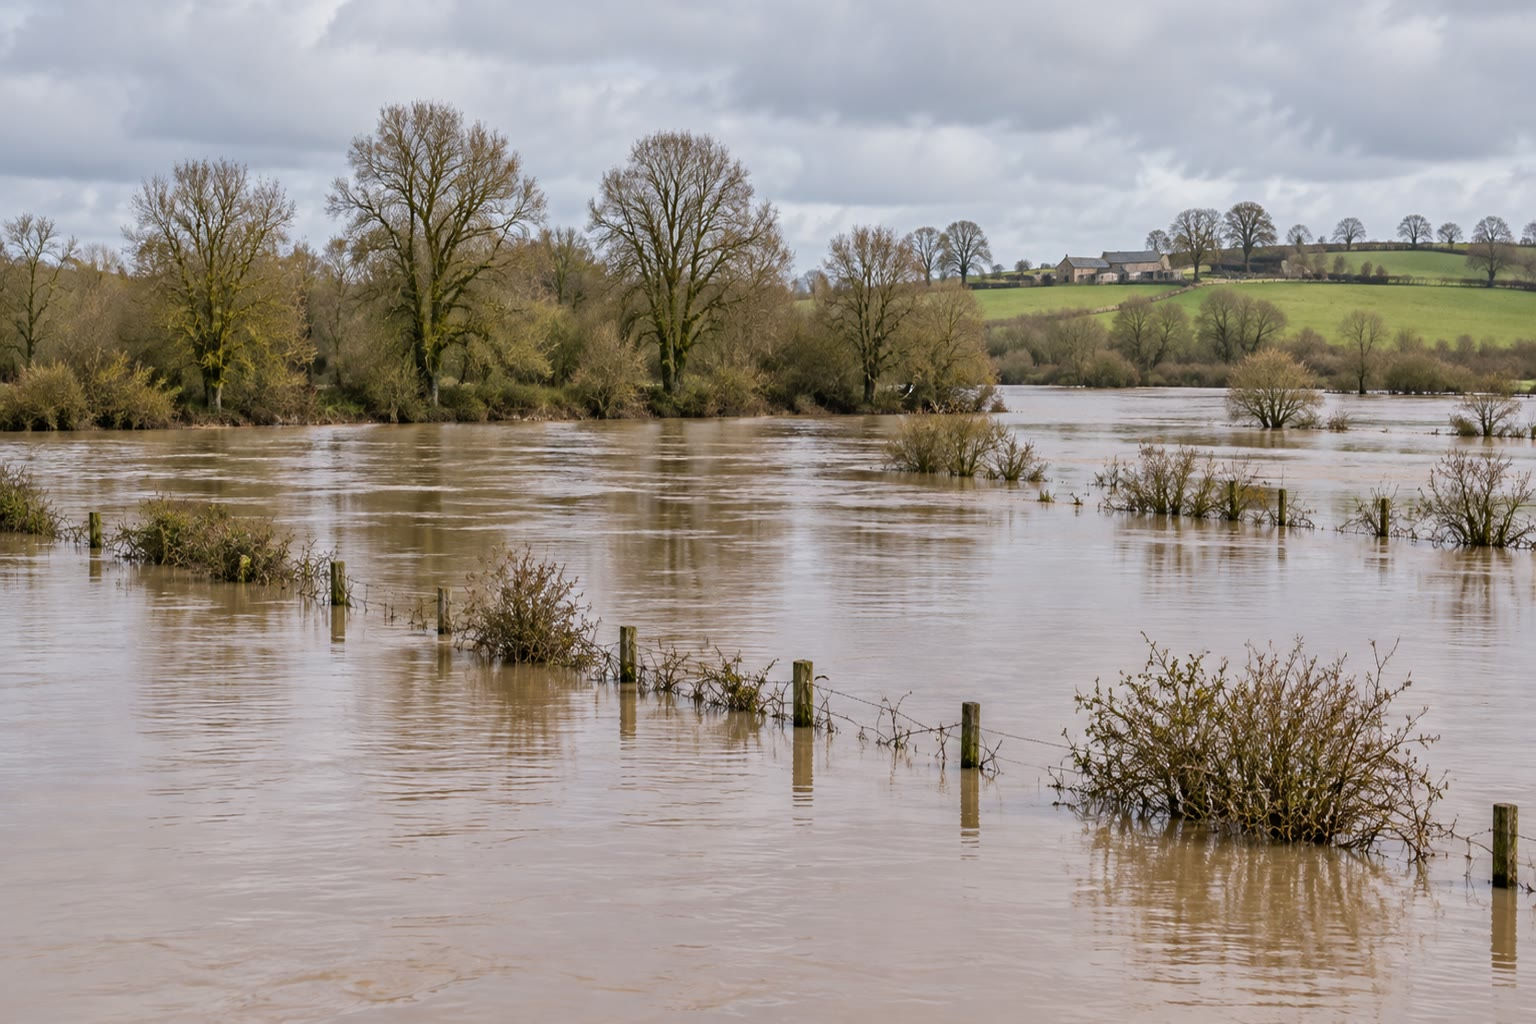
\includegraphics[width=0.5\linewidth]{images/book1/ai/g5-flooded-meadow.jpg}

{\small Un pré sous les eaux de la \omterm{def:g5:water-shapes-the-land:flood}{crue} après des jours de \omterm{def:g4:clouds-rain-snow:precipitation}{pluie}. La ligne
d'arbres marque la berge habituelle de la \omterm{def:g1:landscapes-around-us:water}{rivière}~; la ferme est bâtie sur
une hauteur.}
\end{omfigure}

Une \omterm{def:g1:landscapes-around-us:water}{rivière} en \omterm{def:g5:water-shapes-the-land:flood}{crue} ne fait rien d'étrange~: elle fait ce que les \omterm{def:g1:landscapes-around-us:water}{rivières}
ont toujours fait. La \omterm{def:g5:water-shapes-the-land:flood}{plaine d'inondation} est son territoire. En fait,
c'est la \omterm{def:g1:landscapes-around-us:water}{rivière} qui l'a construite~: chaque \omterm{def:g5:water-shapes-the-land:flood}{crue} laisse derrière elle une
fine couche de \omterm{def:g3:stones-pebbles-sand:sand}{boue} sur les champs, et c'est pourquoi les \omterm{def:g5:water-shapes-the-land:flood}{plaines
d'inondation} ont un sol si riche. Il y a très longtemps, les paysans
d'Égypte attendaient la \omterm{def:g5:water-shapes-the-land:flood}{crue} annuelle du Nil, qui arrosait leurs champs et
leur apportait une \omterm{def:g3:stones-pebbles-sand:sand}{boue} nouvelle.

Mais une \omterm{def:g5:water-shapes-the-land:flood}{crue} est dangereuse pour les gens qui vivent dans la \omterm{def:g5:water-shapes-the-land:flood}{plaine
d'inondation}. Les maisons qui y sont bâties peuvent être envahies par
l'eau, et une eau de \omterm{def:g5:water-shapes-the-land:flood}{crue} rapide peut emporter des voitures et des
personnes. Une ville prudente construit sur les hauteurs et laisse la
\omterm{def:g5:water-shapes-the-land:flood}{plaine d'inondation} aux champs, aux prés et aux parcs. Au
\cref{ch:g5:natural-hazards}, nous verrons comment les gens se préparent
aux \omterm{def:g5:water-shapes-the-land:flood}{crues} et se mettent en sécurité.

\begin{safety}
Ne marche jamais, ne roule jamais à vélo et ne joue jamais dans l'eau d'une
\omterm{def:g5:water-shapes-the-land:flood}{crue}, et ne t'approche jamais d'une \omterm{def:g1:landscapes-around-us:water}{rivière} en \omterm{def:g5:water-shapes-the-land:flood}{crue}~: l'eau est plus forte
et plus profonde qu'elle n'en a l'air, et elle peut cacher des trous et des
bouches d'égout ouvertes. Reste à l'écart jusqu'à ce que les adultes
responsables disent qu'il n'y a plus de danger.
\end{safety}

\section{Exercices}

\begin{exercise}[$\star$]\label{exo:g5:water-shapes-the-land:1}
Nomme le phénomène~: \omterm{def:g5:water-shapes-the-land:weathering}{altération}, \omterm{def:g5:water-shapes-the-land:erosion}{érosion} ou \omterm{def:g5:water-shapes-the-land:deposition}{dépôt}~?
\begin{enumerate}
  \item[(a)] La glace d'une fissure fend une \omterm{def:g3:stones-pebbles-sand:rock}{roche} sur une \omterm{def:g1:landscapes-around-us:landform}{montagne}.
  \item[(b)] Une \omterm{def:g1:landscapes-around-us:water}{rivière} en \omterm{def:g5:water-shapes-the-land:flood}{crue} emporte du \omterm{def:g3:stones-pebbles-sand:sand}{sable} arraché à ses berges.
  \item[(c)] Une couche de \omterm{def:g3:stones-pebbles-sand:sand}{boue} se dépose au fond d'un \omterm{def:g1:landscapes-around-us:water}{lac} calme.
  \item[(d)] Une racine d'arbre fend un mur de pierre.
\end{enumerate}
\end{exercise}

\begin{exercise}[$\star$]\label{exo:g5:water-shapes-the-land:2}
Qu'est-ce que la \omterm{def:g5:water-shapes-the-land:source-mouth}{source} d'une \omterm{def:g1:landscapes-around-us:water}{rivière}~? Son \omterm{def:g5:water-shapes-the-land:source-mouth}{embouchure}~? Qu'est-ce qu'un \omterm{def:g5:water-shapes-the-land:source-mouth}{affluent}~?
\end{exercise}

\begin{exercise}[$\star$]\label{exo:g5:water-shapes-the-land:3}
Range ces parties d'une \omterm{def:g1:landscapes-around-us:water}{rivière} dans l'ordre, de la \omterm{def:g5:water-shapes-the-land:source-mouth}{source} à la \omterm{def:g2:water-on-earth:ocean}{mer}~: les
\omterm{def:g5:water-shapes-the-land:meander}{méandres}~; le \omterm{def:g5:water-shapes-the-land:delta}{delta}~; la \omterm{def:g1:landscapes-around-us:landform}{vallée} étroite en V~; la \omterm{def:g5:water-shapes-the-land:source-mouth}{source}.
\end{exercise}

\begin{exercise}[$\star$]\label{exo:g5:water-shapes-the-land:4}
Vrai ou faux~? Explique.
\begin{enumerate}
  \item[(a)] La \omterm{def:g3:stones-pebbles-sand:rock}{roche} dure ne change jamais.
  \item[(b)] Une \omterm{def:g1:landscapes-around-us:water}{rivière} rapide peut transporter de plus gros cailloux qu'une \omterm{def:g1:landscapes-around-us:water}{rivière} lente.
  \item[(c)] La \omterm{def:g3:stones-pebbles-sand:sand}{boue} la plus fine se dépose en premier, près de la \omterm{def:g5:water-shapes-the-land:source-mouth}{source}.
\end{enumerate}
\end{exercise}

\begin{exercise}[$\star$]\label{exo:g5:water-shapes-the-land:5}
Voici une courbe d'une \omterm{def:g1:landscapes-around-us:water}{rivière} vue de dessus.

\begin{center}
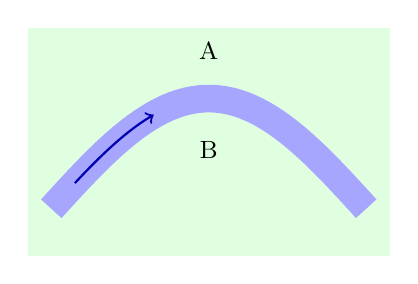
\begin{tikzpicture}[x=1cm, y=1cm, font=\small]
  \fill[green!12] (-0.3,-0.6) rectangle (4.3,2.3);
  \draw[blue!35, line width=10pt] plot[domain=0:4, samples=50]
    (\x,{1.4*sin(\x*45)});
  \draw[blue!70!black, ->, thick] plot[domain=0.3:1.3, samples=20]
    (\x,{1.4*sin(\x*45)});
  \node at (2,2.0) {A};
  \node at (2,0.75) {B};
\end{tikzpicture}
\end{center}
Sur quelle rive, A ou B, la \omterm{def:g1:landscapes-around-us:water}{rivière} use-t-elle la terre~? Sur quelle rive
dépose-t-elle du \omterm{def:g3:stones-pebbles-sand:sand}{sable}~?
\end{exercise}

\begin{exercise}[$\star$]\label{exo:g5:water-shapes-the-land:6}
En \omterm{def:g1:landscapes-around-us:landform}{montagne}, le lit d'une \omterm{def:g1:landscapes-around-us:water}{rivière} est couvert de gros cailloux. Près de la
\omterm{def:g2:water-on-earth:ocean}{mer}, il est couvert de \omterm{def:g3:stones-pebbles-sand:sand}{sable} et de \omterm{def:g3:stones-pebbles-sand:sand}{boue}. Pourquoi~?
\end{exercise}

\begin{exercise}[$\star\star$]\label{exo:g5:water-shapes-the-land:7}
Une \omterm{def:g1:landscapes-around-us:water}{rivière} mesure 600 kilomètres de long. Son cours supérieur occupe le
premier $\frac{1}{6}$ de sa longueur, et son cours moyen la
$\frac{1}{2}$ suivante.
\begin{enumerate}
  \item[(a)] Quelle est la longueur du cours supérieur~? du cours moyen~?
  \item[(b)] Quelle est la longueur du cours inférieur~? Quelle fraction de
        la \omterm{def:g1:landscapes-around-us:water}{rivière} représente-t-il~?
\end{enumerate}
\end{exercise}

\begin{exercise}[$\star\star$]\label{exo:g5:water-shapes-the-land:8}
Regarde de nouveau la photographie du Mamoré prise depuis la station
spatiale, page~\pageref{fig:g5:water-shapes-the-land:mamore}. Que sont les
taches claires à l'intérieur des courbes~? Que sont les \omterm{def:g1:landscapes-around-us:water}{lacs} sombres en
croissant à côté de la \omterm{def:g1:landscapes-around-us:water}{rivière}~? Comment se sont-ils formés~?
\end{exercise}

\begin{exercise}[$\star\star$]\label{exo:g5:water-shapes-the-land:9}
Une ville veut construire une nouvelle école dans les prés verts et plats
qui bordent sa \omterm{def:g1:landscapes-around-us:water}{rivière}, parce que le terrain y est plat et bon marché. Que
dirais-tu au conseil municipal~? Utilise les mots \emph{\omterm{def:g5:water-shapes-the-land:flood}{crue}} et
\emph{\omterm{def:g5:water-shapes-the-land:flood}{plaine d'inondation}}.
\end{exercise}

\begin{exercise}[$\star\star$]\label{exo:g5:water-shapes-the-land:10}
Les fleuves du monde apportent à la \omterm{def:g2:water-on-earth:ocean}{mer} environ 12 milliards de tonnes de
\omterm{def:g3:stones-pebbles-sand:sand}{boue} et de \omterm{def:g3:stones-pebbles-sand:sand}{sable} chaque année.
\begin{enumerate}
  \item[(a)] Combien de tonnes cela fait-il chaque mois, en moyenne~?
  \item[(b)] Un gros camion transporte 10 tonnes. Combien de chargements
        de camion faudrait-il pour transporter la \omterm{def:g3:stones-pebbles-sand:sand}{boue} et le \omterm{def:g3:stones-pebbles-sand:sand}{sable} d'un mois~?
\end{enumerate}
\end{exercise}

\begin{exercise}[$\star\star\star$]\label{exo:g5:water-shapes-the-land:11}
Raconte l'histoire d'un grain de \omterm{def:g3:stones-pebbles-sand:sand}{sable}. Il commence comme une partie d'une
\omterm{def:g3:stones-pebbles-sand:rock}{roche}, haut sur une \omterm{def:g1:landscapes-around-us:landform}{montagne}, et il finit, bien des années plus tard, dans
un \omterm{def:g5:water-shapes-the-land:delta}{delta}. Utilise les mots \emph{\omterm{def:g5:water-shapes-the-land:weathering}{altération}}, \emph{\omterm{def:g5:water-shapes-the-land:erosion}{érosion}} et
\emph{\omterm{def:g5:water-shapes-the-land:deposition}{dépôt}}, et dis ce qui arrive au grain dans le cours supérieur, le
cours moyen et le cours inférieur de la \omterm{def:g1:landscapes-around-us:water}{rivière}.
\end{exercise}
